\documentclass[conference]{IEEEtran}
\IEEEoverridecommandlockouts
% The preceding line is only needed to identify funding in the first footnote. If that is unneeded, please comment it out.
\usepackage{cite}
\usepackage{amsmath,amssymb,amsfonts}
\usepackage{algorithmic}
\usepackage{graphicx}
\usepackage{textcomp}
\usepackage{xcolor}
\usepackage{float}
\def\BibTeX{{\rm B\kern-.05em{\sc i\kern-.025em b}\kern-.08em
    T\kern-.1667em\lower.7ex\hbox{E}\kern-.125emX}}
\begin{document}

\title{Merkle Tree with Post-Quantum Secure Hash: KangarooTwelve and Rescue
\\
}

\author{\IEEEauthorblockN{ Henry Tran}
\IEEEauthorblockA{\textit{Electrical and Computer Engineering} \\
\textit{University of California, San Diego}\\
La Jolla, California \\
het002@ucsd.edu}
\and
\IEEEauthorblockN{Jeffrey Lee}
\IEEEauthorblockA{\textit{Electrical and Computer Engineering} \\
\textit{University of California, San Diego}\\
La Jolla, California \\
jsl019@ucsd.edu}
}

\maketitle

\begin{abstract}
This document is a model and instructions for \LaTeX.
This and the IEEEtran.cls file define the components of your paper [title, text, heads, etc.]. *CRITICAL: Do Not Use Symbols, Special Characters, Footnotes, 
or Math in Paper Title or Abstract.
\end{abstract}

\begin{IEEEkeywords}
component, formatting, style, styling, insert
\end{IEEEkeywords}

\section{Work Completed}

\subsection{Implementations}

\subsubsection{KangarooTwelve} 

In terms of KangarooTwelve, we have been able to get a general implementation completed. We implemented a function that allows us to calculate the permutations that are needed for KangarooTwelve. Furthermore, we were able to get an implementation of TurboSHAKE as well (an implementation for 128 bits and an implementation for 256 bits as well). In terms of the implementation of our permutation function, we followed the paper on FIPS PUB 202, in which laid out the road map into how to build out and generate the permutations. We also followed various psuedocodes and paper on the steps needed in order to create the algorithm. Furthermore, the actual KangarooTwelve was also developed based upon the reference code from authors as well as related papers as well.

\subsubsection{Rescue}

For Rescue-Prime we are in the works of having a working implementation of a hash funciton. So far we are referencing literature and work by the original authors in the development of our implementation. So far we have drafted the Rescue-XLIX permutation logic and are actively working on the sponge construction. We are keeping in mind extendibility and performance to avoid obstacles when porting over to a GPU implementation.

\subsubsection{Merkle Tree}

For Merkle Tree, we have successfully designed and implemented a Merkle Tree data structure that is extensible and easily configurable for various hashes with optimizations kept in mind throughout the implementation. So far, we have successfully operated and tested our Merkle Tree with a SHA256 hash function as a baseline. Furthermore, we have implemented means for proof generation and verification to ensure that we can trace a block of data from a leaf of the Merkle Tree to the root, allowing us to verify the authenticity and integrity of data. Moving forward, we are looking into GPU optimizations with cupy, ways to modularize our implementation further to ensure compatibility with KangarooTwelve and Rescue hash functions, and enabling more features if necessary for testing and experimentation.

\subsection{Experiments and Evaluation}

While we have tested our Merkle Tree using a SHA256 hash function, we have yet to conduct any experiments or evaluation with Kangaroo12 and Rescue. This is still something we are building towards as we continue to finalize our high level implementation of each part. Once we are able to get to a point where we believe the functionality is correct (where that is comparing against public source code (provided by the research groups), or deeper breakdown of paper of each implementation). The hope is that we are able to finish our base configuration within next few days to give us time to properly test our CPU implementation before we move towards GPU.

\subsection{Preliminary Results}

So far we have been able to test verification of our Merkle Tree with SHA256, ensuring that it is able to verify if a valid data block is part of the tree and also catch invalid/corrupted data blocks (shown below). 
Otherwise, We don't have any preliminary results for Kangaroo12 or Rescue as we haven't gotten enough progress to compare results we get from GPU to the CPU.
\begin{figure}[H]
    \centering
    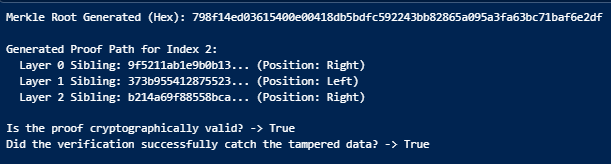
\includegraphics[width=0.5\linewidth]{MerkleTreeSHA256Verification.png}
    \caption{Merkle Tree Verification with SHA256}
    \label{fig:placeholder}
\end{figure}
\section{Challenges and Issues Encountered}

\subsection{Technical difficulties}

A lot of the technical difficulties has come from understanding the hashing functions. Where trying to understand how the function works is a challenge. In terms of with KangarooTwelve, we both have spent a lot of time researching and trying to understand how it is implemented and how documentation on it. However a lot of the documentation seems very spread out where portions of what we want is part of SHA3 (calculating permutations), trying to find documentation on TurboSHAKE and understanding the relation it has in the whole system, and finally getting clear overall understanding of each architecture and the relation towards KangarooTwelve. 
Some more technical issues have emerged with the implementation of Rescue as finding a consistent source to reference for the implementation has been challenging as there are many implementations and components spread out. We have managed to grasp and draft out baseline implementations of the permutation logic and overall structure, but need more time to fully flesh out an implementation that is consistent with the specification.
Merkle Tree has presented relatively little technical difficulties as information on implementation of the Merkle Tree is well documented. The most challenging aspect has been implementing a functioning data structure for Merkle Tree that can be reconfigured and modified with the expectation of having it optimized to the structure and implementation of Kangaroo12 and Rescue. So far, we have had our data structure take in external hash functions and directly hash each node (which is constructed with a basic concatenation operation). This is operational with just a SHA256 hash function but since there are many considerations for Kangaroo12 and Rescue, we would expect for these to be changed or at least modularized for extendibility. Furthermore, we need to take into consideration batching from when we will need to implement hashing with GPU enabled. We have that prepared in our data structure but for now has not impact on the performance.
\subsection{Unexpected experimental behavior}

Currently, we don't have any unexpected experimental behavior given that we haven't progressed enough to give data on experiments being conducted. However, it is likely we will see discrepancies in what should be the output versus what output we do get.

\subsection{Infrastructure or debugging issues}

Currently, we don't necessarily have a lot of infrastructure problems, mainly because we haven't gotten far enough to get to infrastructure problems/debugging issues. Furthermore, we do anticipate that we will have problems with infrastructure, from versions of python, versions of cupy, and versions of various libraries. In terms of debugging, it is likely we will run into that problem once testing begins where we will find out about problems with our code and understanding where the problem may lie.

\subsection{Scope changes or limitations}

In terms of the scope, we think we are relatively on time and should be able to get everything completed in time. However, we do also think that if there are problems that arise we will cut down things. Specifically only doing one version of KangarooTwelve (128 or 256 bits). 

\section{Plans for the next two weeks leading up to the presentation}

\subsection{Remaining milestones}

The remaining milestones that we have is the finish the CPU implementation of each of our hashing functions, finish testing the CPU implementation of our hashing functions, implement the GPU implementation of our hashing functions, and compare results of CPU vs GPU implementations.

\subsection{Planned experiments or evaluations}

Some of the planned experiments/evaluations that we have planned are to evaluate our CPU implementation as to make sure that what we have is correct before moving forward with the GPU implementation. We will also looking to evaluate the timing of the CPU implementation and see the time cost related to it. Furthermore, we plan to experiment with different bit amounts (for KangarooTwelve) as to see if there is a speed vs security difference, and finally to compare timing differences between CPU and GPU for our hashing functions.

\subsection{Writing and presentation preparation}

In terms of the writing and presentation preparation, we don't have much ready yet, but we are closely documentation everything that we have thus far. That includes different documentation that we used to build our functions, reference codes from source implementations, and other documentation regarding our functions. 

\subsection{Division of remaining work}

Currently, we have divided the work through hashing functions. Where Henry will take responsibility primarily for the implementations for KangarooTwelve, while Jeffrey will take responsibility for the implementations for Rescue. In terms of the actual Merkle Tree implementation, we plan to split the work. So currently Jeffrey is getting the base configuration finished so that once we have Rescue and KangarooTwelve finished, we can begin testing on the tree. From there we will switch on and off where Henry will work on getting things setup for different configurations (different hash functions) while also testing the Merkle Tree too to make sure that the tree generation is accurate. Currently, the plan is that we look to get base configurations all done today/tomorrow and begin to start testing over the weekend before starting to implement the GPU version throughout next week. Ultimately, this will still be a lot of work for just two people for this project and we do have some concerns of not being to get everything we want by the end, but we do believe that we can get to a point that best shows the progress we have made.

\end{document}
